\section{Regresión lineal usando datos simulados}

Para propósitos de regresión lineal, escribimos $Y_{e}=\a+\beta X,$ aunque $Y$ rara vez será lineal y podría tener un componente de error o residual, y en ese caso escribimos
\begin{align}
	Y=\a + \beta X + K.
\end{align}


En la ecuación anterior, $K$ es el error, el cuál es una variable aleatoria que supondremos está normalmente distribuida.


Simulemos los datos para $X$ y $Y$ y tratemos de observar como es que los valores estimados $\left( Y_{e} \right)$ difieren del valor real $\left( Y \right)$.


Para $X,$ generamos 100 números aleatorios normalmente distribuidos con media $1.5$ y desviación estándar $2.5$ (pero usted puede tomar otro par de números y experimentar.)


\subsection{Consideraciones}
\begin{enumerate}
	\item Para el valor $(Y_{e}),$ supondremos una ordenada al origen $\a=2$ y una pendiente $\beta=0.3$. 
	
	\item
	Posteriormente, calcularemos los valores óptimos de $\a$ y $\beta$, usando los datos simulados y veremos como cambia la eficacia del modelo.
	
	\item
	Para el valor actual $Y$, adicionamos un término residual, que no es otra cosa que una variable normalmente distribuida con media $\mu=0$ y desviación estándar de $\sigma=0.5$.
\end{enumerate}


[,]{\texttt{fittingLinearRegression.py}}
\begin{lstlisting}[language=Python]
	import pandas as pd
	import numpy as np
	
	np.random.seed(1234)
	
	x=2.5*np.random.randn(100)+1.5
	res=.5*np.random.randn(100)+0
	ypred=2+.3*x
	yact=2+.3*x+res
	xlist=x.tolist()
	ypredlist=ypred.tolist()
	yactlist=yact.tolist()
	df=pd.DataFrame({'Input_Variable(X)':xlist,'Predicted_Output(ypred)':ypredlist,'Actual_Output(yact)':yactlist})
	print(df.head())
	
	
	import matplotlib.pyplot as plt
	
	% x=2.5*np.random.randn(100)+1.5
	% res=.5*np.random.randn(100)+0
	% ypred=2+.3*x
	% yact=2+.3*x+res
	
	ymean=np.mean(yact)
	yavg=[ymean for i in range(1,len(xlist)+1)]
	
	plt.plot(x,ypred)
	plt.plot(x,yact,'ro')
	plt.plot(x,yavg)
	plt.title('Actual vs Predicted')
\end{lstlisting}

[,]{} 
\begin{lstlisting}[language=Python]
	Actual_Output(yact)  Input_Variable(X)  Predicted_Output(ypred)
	0             2.949179           2.678588                 2.803576
	1             1.840035          -1.477439                 1.556768
	2             3.776326           5.081767                 3.524530
	3             2.358159           0.718370                 2.215511
	4             2.151703          -0.301472                 1.909558
\end{lstlisting}


\begin{center}
	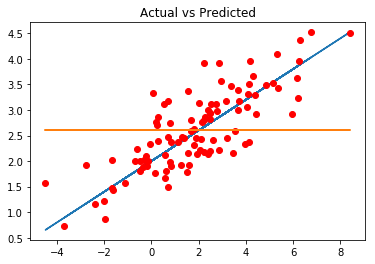
\includegraphics[width=10cm,keepaspectratio=true]{./images/actualVsPredicted.png}
	% actualVsPredicted.png: 0x0 pixel, 300dpi, 0.00x0.00 cm, bb=
\end{center}



En la gráfica anterior, la linea horizontal representa la \emph{media} de los datos.


En caso de que no tuviéramos algún otro modelo predictivo, nuestra mejor elección sería la \emph{media aritmética}.


Otro punto para pensar es en como juzgar la eficiencia de nuestro modelos. 

Si usted pasa cualquier dato conteniendo dos variables, una de entrada y otra de salida, el programa de estadística generara algunos valores $\a,\beta.$



¿Pero cómo entender que esos valores que se nos están dando son un buen modelo?

\subsection{Suma de Cuadrados Total}
\begin{align}
	SST = \sum\left( Y_{i}-\bar{Y} \right)^{2}
\end{align}

donde $\bar{Y}$ es el valor promedio de $Y_{1}, Y_{2},...$, los valores reales de $Y.$


\subsection{Suma de Cuadrados de Regresión}

\begin{align}
	SSR = \sum\left( Y_{e,i}-\bar{Y} \right)^{2}
\end{align}
donde $\bar{Y}$ es el valor promedio de $Y_{1}, Y_{2},...$, los valores reales de $Y,$ mientras que $Y_{e,i}$ son los valores predichos por el modelos para cada $Y_{i}.$


\subsection{Suma de Cuadrados de Diferencia}
\begin{align}
	SSD = \sum\left( Y_{i}-Y_{e,i} \right)^{2}
\end{align}



Recordemos que $Y_{e}=\a + \beta X$, con $\beta$ definida por \eqref{beta} y $\a$ por \eqref{alfa}.



Utilizando estas identidad se puede demostrar que
\begin{align}
	SST = SSR +SSD.
\end{align}



\begin{itemize}
	\item $SSR$: diferencia explicada por el modelo;
	\item $SSD$: diferencia no explicada por el modelo;
	\item $SST$: error total.
\end{itemize}




\begin{observacion}
	Entre mayor sera la proporción de $SSR:SST$, mejor será el modelo.
\end{observacion}


\subsection{Coeficiente de determinación}
\texttt{R-cuadrado: }
\begin{align}
	R^{2}=\dfrac{SSR}{SST}
\end{align}


Como $SSR\leq SST,$ entonces $0\leq R^{2} \leq 1$, y entre más cercano sea a $1$ mejor será el modelo.



$R^{2}$ es un buen indicador de que una regresión lineal será efectiva.


En el script \texttt{fittingLinearRegression.py}, podemos agregar el siguiente pedazo de código para calcular el valor $R^{2}$.

[,]{\texttt{rCuadrada.py}}
\begin{lstlisting}[language=Python]
	df['SSR']=(df['Predicted_Output(ypred)']-ymean)**2
	df['SST']=(df['Actual_Output(yact)']-ymean)**2
	SSR=df.sum()['SSR']
	SST=df.sum()['SST']
	SSR/SST
\end{lstlisting}


El valor obtenido es $a\approx 0.65$, que es algo bueno. Sin embargo, los valores $\a=2, \beta=0.3$ para $Y_{e}$ pueden que no sean los mejores.
